\documentclass[notitlepage]{revtex4-1}
\usepackage{geometry}
\usepackage{graphicx}
\usepackage{times}
\usepackage{physics}   % for simple physics notation
\usepackage{bm}        % for math
\usepackage{amssymb}   % for math
\usepackage{amsmath}
\usepackage{subfigure}
\usepackage{color}
\usepackage{float}
\usepackage{enumitem}
\usepackage[export]{adjustbox}
\usepackage{comment}
\usepackage{listings}
\usepackage{CJK}
\usepackage{graphicx}
\usepackage{booktabs}
\usepackage{hyperref}
\newcommand{\hilight}[1]{\colorbox{red}{#1}}
%\usepackage{physics}
%\usepackage{enumerate}
%\usepackage{booktabs} % not allowed in Revtex4.1
\begin{document}
\begin{CJK}{UTF8}{bsmi}
\title{First Principle 2017-Fall  midterm Solution}
%\input author_list.tex       % D0 authors (remove the first 3 lines
                             % of this file prior to submission, they
                             % contain a time stamp for the authorlist)
                             % (includes institutions and visitors)
\author{Kai-Hsin Wu (吳愷訢)}
\email{r05222003@ntu.edu.tw}
\affiliation{Department of Physics and Center for Theoretical Sciences, National Taiwan University, Taipei 10607, Taiwan}

%\date{\today}
\maketitle

\begin{enumerate}	
	\item Al band structure using GGA calculation and free-electron band structure.
	\begin{figure}[!h]
		\begin{minipage}{\textwidth}
			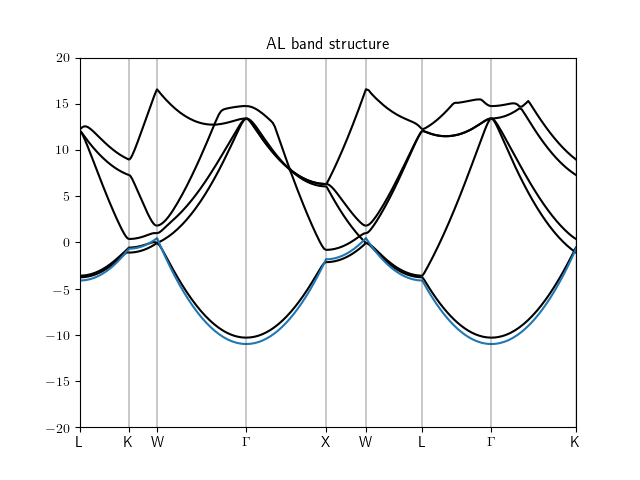
\includegraphics[width=.6\textwidth]{{Material/q1/Al}.png}
			\label{fig:Al-free}
			\caption{Al band structure and free-electron band}
		\end{minipage}	
	\end{figure}
	
	In match the free electron band, we have to consider also the work function $W$ (or equivalent the vacuum potential ) of Al, in which the calculation gives : $W_{Al} = 3.207 eV$  
	
	\item Consider 1D case of KS ansatz. To derive the KS potential from the known density, we start with KS equation:
		\begin{equation}
			\left[ -\frac{1}{2} \frac{\partial^2}{\partial x^2} + v_s(x)\right] \phi_i(x) = \epsilon_i \phi_i(x)
		\end{equation}
		
		In here we set $\hbar$ and mass $m$ as 1.  
	
		Since there is a freedom to choose the basis, we can choose a basis that is real such that $\phi_i^* = \phi_i$. In which we can express the density and the kinetic density $\tau_L$ and $\tau$ as :
		\begin{align}
			\rho(x) &= \sum_{i} \phi(x)^2 \\
			\tau_L &= -\frac{1}{2} \sum_i \phi_i(x) \frac{\partial^2}{\partial x^2} \phi_i(x) \\
			\tau   &= \frac{1}{2} \sum_i |\frac{\partial}{\partial x}\phi_i(x)|^2 \\
			\tau_L &= \tau - \frac{1}{4} \frac{\partial^2}{\partial x^2} \rho(x)
		\end{align}
		
		 First, we multiply KS equation with $\phi_i$ and sum over $i$:
		\begin{align}
			\tau_L + v_s(x)\rho(x) = \sum_i \epsilon_i \phi_i(x)^2 
		\end{align}		
		then take derivation: 
		\begin{align}
			\frac{\partial}{\partial x}\tau_L + v_s(x)\frac{\partial}{\partial x}\rho(x) + \rho(x) \frac{\partial}{\partial x} v_s(x)= 2\sum_i \epsilon_i \phi_i(x) \frac{\partial}{\partial x} \phi_i(x) 
		\end{align}			 
		
		Now return to equation (1) and multiply by $2\frac{\partial}{\partial x}\phi_i(x)$ and sum over i:
		\begin{align}
			-\sum_{i} \frac{\partial^2}{\partial x^2} \phi_i(x) \frac{\partial}{\partial x} \phi_i(x) + v_s(x)\frac{\partial}{\partial x}\rho(x) = 2\sum_i \epsilon_i \phi_i(x) \frac{\partial}{\partial x} \phi_i(x)
		\end{align}
		
		combine with equation (7) and (8), we have :
		\begin{align}
			&\frac{\partial}{\partial x} \tau_L + \sum_i \frac{\partial^2}{\partial x^2} \phi_i(x) \frac{\partial}{\partial x} \phi_i(x) + \rho(x) \frac{\partial }{\partial x} v_s(x) \\
			&=\frac{\partial}{\partial x} \tau_L + \frac{\partial}{\partial x} \tau + \rho(x) \frac{\partial }{\partial x} v_s(x)  = 0 
		\end{align} 
		
		With given density $\rho(x)$:
		\begin{equation}
			\rho(x) = Ae^{-\alpha x^2}
		\end{equation}
		the kinetic energy densities are obtained:
		\begin{align}
			\tau &= \frac{1}{2} A \alpha^2 x^2 e^{-\alpha x^2} \\
			\tau_L &= \frac{A\alpha}{2} e^{-\alpha x^2} \left[ 1 - \alpha x^2 \right]
		\end{align}
		insert (12),(13) into (10) we have :
		\begin{align}
			\rho(x) \frac{\partial}{\partial x} v_s(x) = \alpha^2 x \rho(x)
		\end{align}
		
		Thus we have derived the potential with constant $c$:
		\begin{equation}
			v_s(x) = \frac{\alpha^2}{2} x^2 + c
		\end{equation}
		
		Finally, the normalization constant A can be derived with :
		\begin{align}
			\int_{-\infty}^{\infty} \rho(x) &= 1 \\
			A\int_{-\infty}^{\infty} e^{-\alpha x^2} &= A\sqrt{\frac{\pi}{\alpha}} = 1
		\end{align}		
		\begin{align}
			A = \sqrt{\frac{\alpha}{\pi}}
		\end{align}			
		
	\item Car-Parrinelo EOM
	
		The Car-Parrinelo lagrangian:
		\begin{align}
				L = \sum_{i} \frac{1}{2} \mu \int |\dot{\phi_i}(r)|^2 dr + \sum_{I} \frac{1}{2} M_I \dot{R_I}^2 - E \left[{\phi_i},{R_i}\right] - \sum_{ij} \Lambda_{ij} \int \phi_i(r) \phi_j(r) dr - \delta_{ij}
		\end{align} 
		 To impose the orthonmality, we add a term with lagrangian multiplier $\Lambda_{ij}$. With the Euler-Lagrangian equation:
		 \begin{equation}
		 	\frac{d}{dt} \frac{\partial L }{\partial \dot{q}} = \frac{\partial L}{\partial q}
		 \end{equation} 
		 The equation of motion of electronic and ionic DOF can be derived as:
		 \begin{align}
		 	\mu \ddot{\phi_i}(r) &= -\sum_{j} \Lambda_{ij} \phi_j(r) - \frac{\partial E[{\phi_i},{R_I}]}{\partial \phi_i} \\
		 	M_I \ddot{R_I} &= \frac{-\partial E[{\phi_i},{R_I}]}{\partial R_I}
		 \end{align}
		 
	
	\clearpage
	\item GGA, GGA+U of MnO in AF-II
		The crystal and magnetic structure of MnO in AF-II:
		\begin{figure}[!h]
		\centering 
		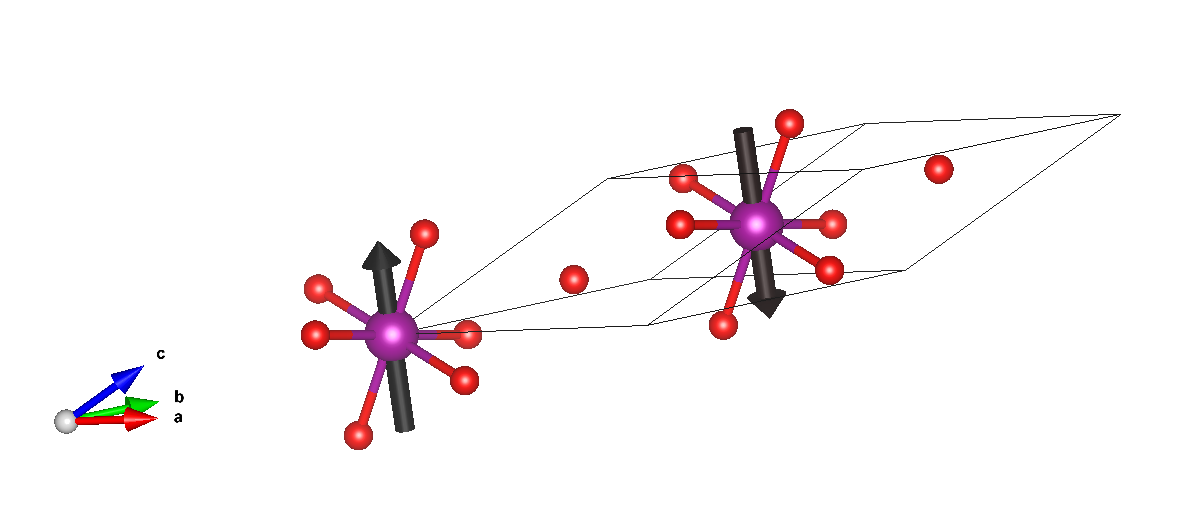
\includegraphics[width=14cm]{{Material/q4/MnO-AFII}.png}
		\caption{MnO in AF-II, (\textbf{purple}: \textit{Mn} atoms carry magnetic moment; \textbf{red}: non-magnetic \textit{O} atoms) }
		\label{fig:MnOAFII-latt}
		\end{figure}
	
		\begin{itemize}
		\item GGA 
		\begin{enumerate}[label=(\arabic*)]
			\item the band structure and total DOS, the energies are shifted by fermi energy $E_{f} = 5.2304 eV$ to zero.
			\begin{figure}[!h]
				\centering
				\begin{minipage}{.5\textwidth}
					\centering
					\includegraphics[width=9cm]{{Material/q4/Result_GGA/gap}.png}
					\caption{MnO-AFII band-structure }
					\label{fig:MnOAFII-band}
				\end{minipage}%
				\begin{minipage}{0.5\textwidth}
					\centering
					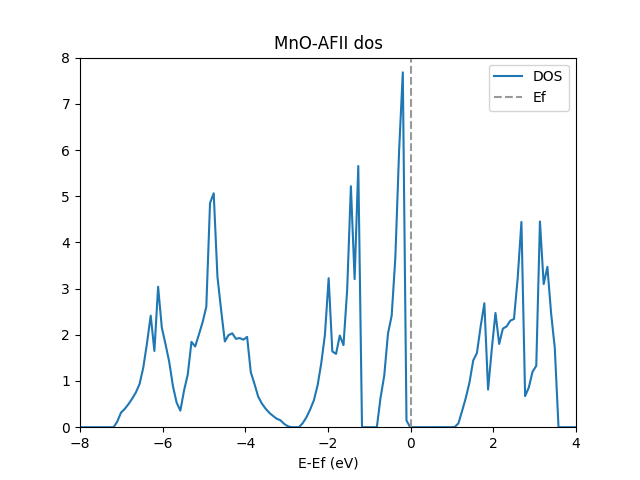
\includegraphics[width=9cm]{{Material/q4/Result_GGA/MnO-totdos}.png}
					\caption{MnO-AFII density of state}
					\label{fig:MnOAFII-dos}
				\end{minipage}
			\end{figure}
			\begin{figure}[!h]
				\centering
				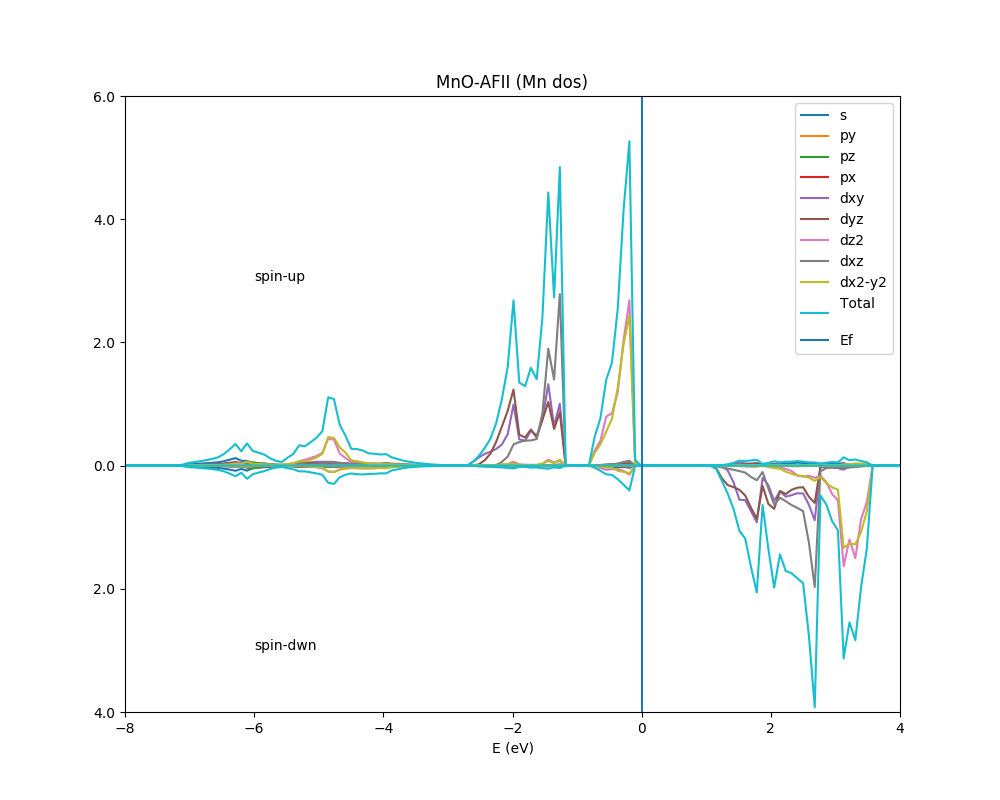
\includegraphics[width=11cm]{{Material/q4/Result_GGA/MnO-AFII_Mn}.png}
				\caption{Mn in MnO density of state}
				\label{fig:Mn-dos}
			\end{figure}
		
			Energy gap $E_g$ ,total magnetic moment $m$ and Mn moment $m_{Mn}$:
			\begin{align*}
			E_g &= 0.918700 eV \\ 
			m  &= 0.0000 \mu_{B} \\
			m_{Mn} &= 4.199 \mu_{B}
			\end{align*}
			
		\end{enumerate}
	
		\clearpage
		
		\item GGA+U 
		\begin{enumerate}[label=(\arabic*)]
			
			\item the band structure and total DOS, the energies are shifted by fermi energy $E_{f} = 4.0271/ eV$ to zero.
			\begin{figure}[!h]
				\centering
				\begin{minipage}{.5\textwidth}
					\centering
					\includegraphics[width=9cm]{{Material/q4/Result_GGA+U/gap}.png}
					\caption{MnO-AFII band-structure GGA+U}
					\label{fig:MnOAFII-band+U}
				\end{minipage}%
				\begin{minipage}{0.5\textwidth}
					\centering
					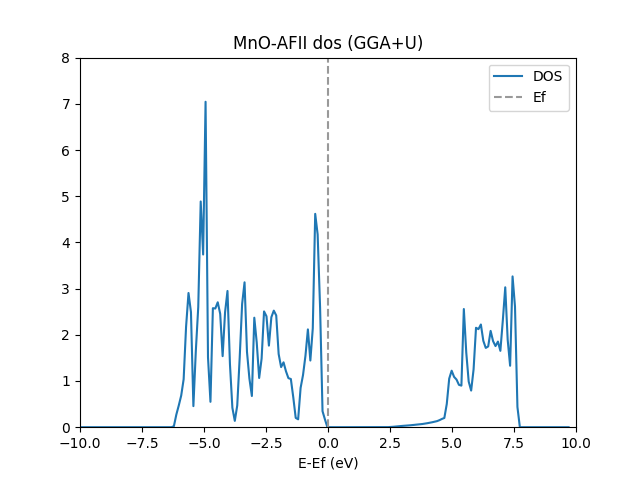
\includegraphics[width=9cm]{{Material/q4/Result_GGA+U/MnO-totdos-gga+u}.png}
					\caption{MnO-AFII density of state GGA+U}
					\label{fig:MnOAFII+u-dos}
				\end{minipage}
			\end{figure}
			
			\begin{figure}[!h]
				\centering
				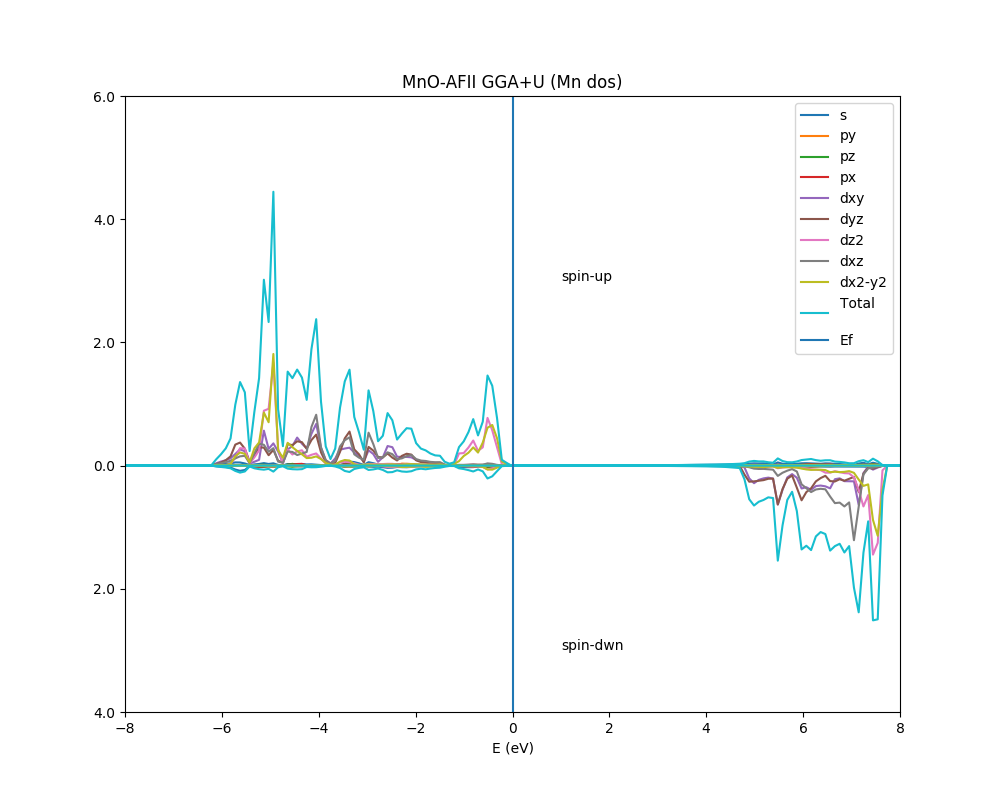
\includegraphics[width=10cm]{{Material/q4/Result_GGA+U/MnO-AFII_Mn-gga+u}.png}
				\caption{Mn in MnO density of state GGA+U}
				\label{fig:Mn-dos+u}
			\end{figure}
			
			Energy gap $E_g$ ,total magnetic moment $m$ and Mn moment $m_{Mn}$:
			\begin{align*}
			E_g &= 2.318900 eV \\ 
			m  &=  0.0000 \mu_{B}   \\
			m_{Mn} &= 4.686 \mu_{B}
			\end{align*}
			
			By apply $U_{eff}$ on Mn, we decouple the Mn and O energy part, as a result, the AF magnetic property contributed form Mn can be calculate more accurate. 
		\end{enumerate}
	
	\end{itemize}
	

	
	\item Finite difference algorithms. 
	
		In the following, we evaluate the harmonic oscillator with "Euler" , "Predictor-Corrector" and "Velocity-verlet" method.
		\begin{enumerate}[label=(\alph*)]
		\item Euler method with different $dt$ (in unit of $\pi$) for initial condition $x(0) = 1$,$v(0) = 0$ :
			\begin{figure}[!h]
				\begin{minipage}{\textwidth}
					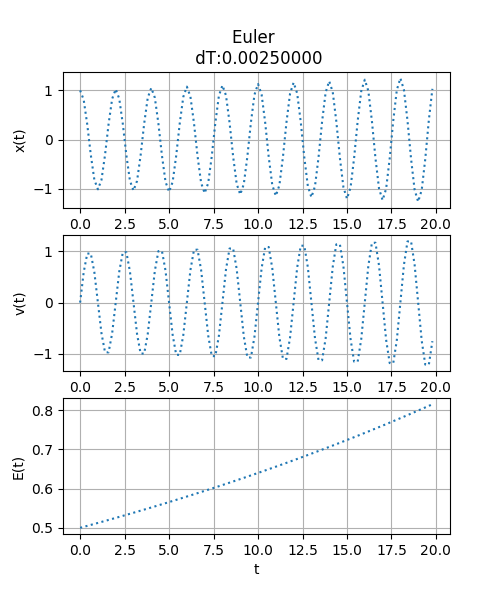
\includegraphics[width=.4\textwidth]{{Material/q5/Euler-2.5000E-03}.png}
					\label{fig:eu-3}
					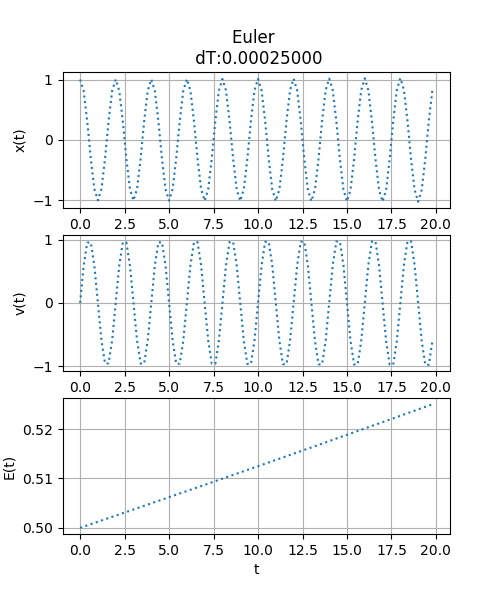
\includegraphics[width=.4\textwidth]{{Material/q5/Euler-2.5000E-04}.png}
					\label{fig:eu-4}
					\caption{Euler method, $dt = 2.5 \times 10^{-3} (left)$ and $dt = 2.5 \times 10^{-4} (right)$ }
				\end{minipage}	
			\end{figure}

		compare the result with (a), we can see that  reducing the update time interval, the energy still not conserved, but the error is decreased. 
		\clearpage

		\item Euler method compare with Predictor-Corrector method with $dt = 2.5 \times 10^{-3}$ (in unit of $\pi$), $x(0) = 1$,$v(0) = 0$ 
			\begin{figure}[!h]
				\begin{minipage}{\textwidth}
					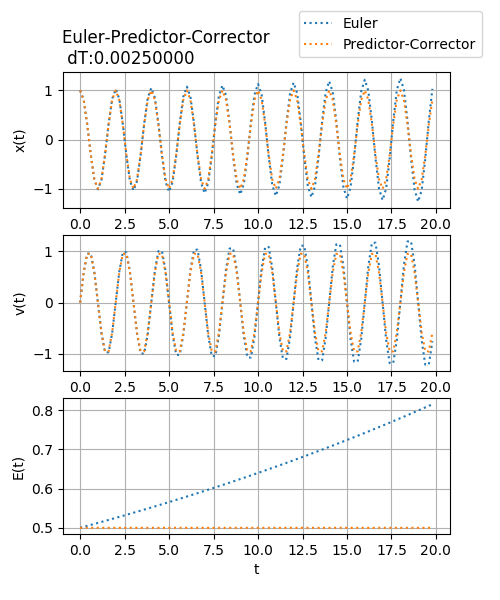
\includegraphics[width=.5\textwidth]{{Material/q5/Euler-Predictor-Corrector_2.5000E-03}.png}
					\label{fig:eupc-3}
					\caption{Euler v.s. Predictor-Corrector method , $dt = 2.5 \times 10^{-3}$}
				\end{minipage}	
			\end{figure}
		

		compare the result with (a), we can see that with the same update time interval ($dt$), we can see that the energy increment error is significantly reduced.  
		\clearpage
		\item Euler method compare with Velocity-Verlet method with $dt = 2.5 \times 10^{-3}$ (in unit of $\pi$), $x(0) = 1$,$v(0) = 0$ 
		
			\begin{figure}[!h]
				\begin{minipage}{\textwidth}
					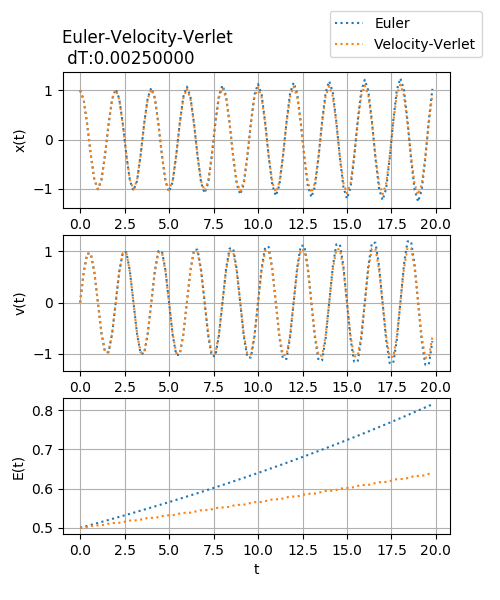
\includegraphics[width=.5\textwidth]{{Material/q5/Euler-Velocity-Verlet_2.5000E-03}.png}
					\label{fig:euvv-3}
					\caption{Euler v.s. Velocity-Verlet method , $dt = 2.5 \times 10^{-3}$}
				\end{minipage}	
			\end{figure}
		
		compare the result with (a), we can see that with the same update time interval ($dt$), we can see that the energy increment error is reduced.  

		\end{enumerate}

\end{enumerate}


\end{CJK}

\bibliographystyle{apsrev4-1}
\bibliography{ref}
	

\end{document}

